\documentclass[
%  master,
%  program=infpvs,
%  printversion,
  biblatex,
%  language=english,
%  font=sans,
  figures=false,
  glossaries,
  index
]{kidiplom}

\title{Algoritmy pro problém obchodního cestujícího}
\title[english]{Algorithms for the travelling salesman problem}

\author{Kateřina Sáňková}

\supervisor{Mgr. Petr Osička, Ph.D.}

\yearofsubmit{\the\year}

\annotation{Anotace - jeden odstavec}

\annotation[english]{Anotace anglicky}

\keywords{problém obchodního cestujícího;}
\keywords[english]{travelling salesman problem;}

\thanks{Děkuji, děkuji, děkuji.}

%% Cesta k souboru s bibliografií pro její sazbu pomocí BibLaTeXu
%% (zvolenou nepovinným parametrem biblatex makra
%% \documentclass). Použijte pouze při této sazbě, ne při (výchozí)
%% sazbě v prostředí thebibliography.
\bibliography{bibliografie.bib}

%% Další dodatečné styly (balíky) potřebné pro sazbu vlastního textu
%% práce.
\usepackage{lipsum}
\usepackage{longtable}
\usepackage[ruled, noend]{algorithm2e} 
\usepackage{enumitem}
\usepackage{tikz}
\usepackage{caption}

\begin{document}
%% Sazba úvodních stran -- titulní, s bibliografickými údaji, s
%% anotací a klíčovými slovy, s poděkováním a prohlášením, s obsahem a
%% se seznamy obrázků, tabulek, vět a zdrojových kódů (pokud jejich
%% sazba není vypnutá).
\maketitle

%% Vlastní text závěrečné práce. Pro povinné závěry, před přílohami,
%% použijte prostředí kiconclusions. Povinná je i příloha s obsahem
%% přiloženého datového média.

%% -------------------------------------------------------------------

\newcommand{\BibLaTeX}{\textsc{Bib}\LaTeX}

\section{Teorie}
Problém obchodního cestujícího je úzce spjatý s \textit{teorií grafů} a proto je potřeba si na úvod zavést některé z jejich základních pojmů.

\subsection{Graf}
Graf je jedna ze základních reprezentací prvků množiny objektů a jejich vzájemných propojení. Takovým objektům budeme říkat \textit{vrcholy} (někdy také \textit{uzly}) a propojením \textit{hrany}. Uvažujeme-li orientaci hran, pak říkáme, že je graf \textit{orientovaný}, jinak \textit{neorientovaný}.

\begin{definition}[Neorientovaný graf]
\textit{Neorientovaný graf} je dvojice $\langle V, E \rangle$, kde $V$ je neprázdná množina vrcholů a $E \subseteq \{\{u, v\} \mid u, v \in V$, $u \neq v \}$ je množina (\textit{neorientovaných}) hran.

$u, v$ nazýváme \textit{koncové uzly} hrany.
\end{definition}
 
V některých situacích nás bude zajímat počet hran, kterým je jistý uzel koncovým. Tomuto číslu budeme říkat \textit{stupeň vrcholu} $u$ a budeme ho značit $deg(u)$. Důležité bude také následující tvrzení.

\begin{theorem}\label{theorem:degree}
V každém grafu $G=\langle V, E \rangle$ platí, že $\sum_{v \in V} deg(v) = 2 |E|$.
\end{theorem}

U problému obchodního cestujícího také chceme, aby hrany vstupních grafů měly nějakou váhu. Tu jim přiřazuje tzv. \textit{hranové ohodnocení} definované následovně:
$$w : E \rightarrow D$$
kde $w$ je \textit{hranové ohodnocení}, $E$ je množina hran příslušného grafu a $D$ je nějaká množina hodnot.\newline

Dále je vstupem tzv. \textit{úplný} graf. V takovém grafu platí, že každé dva jeho vrcholy  jsou spojeny hranou.

\subsubsection{Cestování v grafech}
Důležitou oblastí práce s grafy je cestování v nich. Vychází se z toho, že se z jednoho uzlu můžeme přemístit k druhé. právě když mezi nimi existuje hrana (v případě orientovaných grafů musí mít ještě hrana správný směr). Jednou z úloh o cestování je právě problém obchodního cestujícího.


Základním pojmem, od kterého budeme odvozovat další, je \textit{sled}.


\begin{definition}
\textit{Sledem} v grafu $G=\langle V, E \rangle$ rozumíme posloupnost $v_0, e_1, v_1, e_2, v_2, \cdots, e_n, v_n$, kde $\forall i \in \{0,\cdots, n\} \ v_i \in V$ a $\forall j \in \{1, \cdots, n\} \ e_j \in E$.
\end{definition}


Sled nazýváme
\begin{itemize}
\item \textit{uzavřený}, pokud $v_0 = v_n$
\item \textit{tah}, pokud $\forall k, l \in \{1, \cdots, n\}$, kde $k \neq l$, $e_k \neq e_l$ (neopakují se hrany)
\item \textit{cesta}, pokud $\forall k, l \in \{0, \cdots, n\}$, kde $k \neq l$, $v_k \neq v_l$ (neopakují se vrcholy)
\item \textit{kružnice}, pokud je \textit{cestou}, ale $v_0 = v_n$
\end{itemize}

Speciální druh tahu je tzv. \textit{eulerovský tah}. Pro něj platí, že vede přes všechny vrcholy a každá hrana se v něm vyskytuje právě jednou. 

\begin{theorem}\label{theorem:eulerianCircout}
Pokud je neorientovaný graf souvislý a všechny jeho vrcholy mají sudý stupeň, pak v něm existuje uzavřený eulerovský tah.
\end{theorem}

Pro TSP je ještě klíčový termín \textit{hamiltonovská kružnice}. Tou rozumíme takovou kružnici v grafu, která vede přes všechny jeho vrcholy.
\newline

Některé z algoritmů v knihovně jsou založené na hledání tzv. \textit{minimální kostry grafu} . Před zavedením tohoto pojmu je ještě nutné si definovat, co je to \textit{souvislý graf} a \textit{podgraf} grafu.

\begin{definition}[Souvislý graf]
Neorientovaný graf $G=\langle V, E \rangle$ nazýváme \textit{souvislý}, pokud $\forall u,v \in V$ existuje sled (viz později) z $u$ do $v$.
\end{definition}

\begin{definition}[Podgraf]
Graf $G_2=\langle V_2, E_2 \rangle$ nazýváme \textit{podgraf} grafu $G=\langle V, E \rangle$, právě když $V_2 \subseteq V$ a $E_2 \subseteq  E$.
\end{definition}

\begin{definition}[Kostra grafu]
Kostra neorientovaného grafu je jeho souvislý podgraf, který obsahuje všechny jeho vrcholy a nevyskytují se v něm žádné kružnice (viz později).
\end{definition}

Pokud mají hrany původního grafu přiřazené váhy příslušným hranovým ohodnocením $w$, potom můžeme uvažovat o \textit{minimální kostře grafu}. Tou budeme rozumět právě takovou kostru $MSP = \langle V, E' \rangle$, která bude mít mezi ostatními minimální součet  $\sum_{e \in E'} w(e)$.

\subsection{Problém}
Obecně lze problémy, u kterých je rozumné chtít pro řešení použít počítač, definovat pomocí množiny vstupů $In$, množiny možných výstupů $Out$ a funkce $p : In \rightarrow Out$, která každému vstupu přiřazuje odpovídající výstup. Tedy $P = \langle In, Out, p \rangle$.

\textit{Optimalizační problémy} jsou takové problémy, kde pro vstup existuje víc možných řešení a jejich úlohou je najít mezi nimi najít které bude mezi nimi buď minimální nebo maximální vzhledem k nějaké předem dané funkci.

Tyto problémy se dají charakterizovat 
\begin{itemize}
\item množinou vstupů $In$
\item funkcí $sol : In \rightarrow 2^{Out}$, která každému vstupu přiřadí množinu \textit{přípustných řešení}
\item funkcí $cost : In \times Out \rightarrow \mathbb{Q}$, která vstupu a jeho přípustnému řešení přiřazuje \textit{cenu} toho řešení
\item $goal$, které je buď $\min$ nebo $\max$
\end{itemize}

Podle hodnoty $goal$ se problému říká \textit{minimalizační} nebo \textit{maximalizační}. \textit{Optimálním řešením} pro vstup $x \in In$ pak označujeme takové řešení $y \in sol(x)$, pro které platí, že $cost(x, y) = goal\{cost(x, y') \mid y' \in sol(x)\}$. Cenu takového řešení značíme $OPT(x)$.

\sloppy Při hledání algoritmu, které řeší takový problém zvažujeme jeho \textit{správnost} a \textit{optimalitu}. Řekneme, že algoritmus $A$ pro problém $P$ je \textit{správný}, pokud $\forall x~\in~In, A(x) \in sol(x)$. \textit{Optimální} je navíc pokud $\forall x \in In$ je $A(x)$ optimální řešení.

\sloppy Některé optimální algoritmy bývají ale časově náročné, často se proto hledají algoritmy, které nevydají pokaždé optimální řešení, ale pouze přibližné. Těmto algoritmům se říká \textit{aproximační}.

Mějme takový algoritmus $A$. Pro každý vstup $x \in In$ můžeme definovat \textit{aproximační faktor} jako $$R_A(x) = \max\{\frac{cost(x, A(x))}{OPT(x)},\frac{OPT(x)}{cost(x, A(x)}\}$$

Pro samotný algoritmus můžeme také definovat jeho aproximační faktor, vzhledem k nějaké funkci $F$ mapující vstupy na přirozená čísla, a to následovně $$R_A(n)~=~\max\{R_A(x) \mid x \in In, F(x) = n\}$$

$A$ můžeme označit za $f(n)$\textendash aproximační algoritmus, pokud $\forall n \in \mathbb{N}$ platí $R_A(n) \le f(n)$. Jinými slovy, pokud u algoritmu známe jeho aproximační faktor, pak se můžeme spolehnout, že pro každý vstup velikosti $n$ dostaneme v nejhorším případě $f(n)$\textendash krát horší výsledek vůči optimu.
\newline

Další významnou množinou problémů jsou \textit{rozhodovací problémy}. Ty se vyznačují tím, že množina výstupů je omezena jen na \textsc{Ano} a \textsc{Ne}.

Každý optimalizační problém má svoji \textit{rozhodovací verzi}. Místo, aby na vstupu byla pouze instance problému $x \in In$, přidá se navíc ještě číslo $k \in \mathbb{Q}$. Pokud je $k \ge OPT(x)$, u minimalizačního problému, nebo $k \le OPT(x)$, u maximalizačního, pak je výsledkem  \textsc{Ano}, jinak \textsc{Ne}.

\subsubsection{Složitost}
Na začátku je třeba si zavést třídy \textbf{P} a \textbf{NP}. Algoritmy, které spadají do třídy \textbf{P} jsou řešitelné deterministickými stroji v polynomiálním čase a bereme je za praktický zvládnutelné. Na nedeterministických strojích můžeme řešit v polynomiálním čase \textbf{NP} problémy. U těchto strojů předpokládáme, že z možných kroků provede vždy ten žádaný a dostane se tak ke správnému výsledku bez nutnosti zkoušet všechny možnosti. Jistě platí $\textbf{P} \subseteq \textbf{NP}$, jelikož deterministické stoje jsou speciálním případem nedeterministických, které pouze nevyužívají možnosti nedeterministického výběru.

Některé rozhodovací problémy mají navíc tu vlastnost, že jsou na ně polynomiálně redukovatelné všechny rozhodovací problémy v \textbf{NP}. To znamená, že pro každý vstup libovolného problému $P_1$ můžeme v polynomiálním čase najít vstup pro $P_2$, který bude vracet stejnou odpověď, jakou by vrátil $P_1$ na původní vstup. Problémům s touto vlastností se říká \textit{\textbf{NP}\textendash těžké}.

Pokud jsou navíc \textbf{NP}, říká se jim \textit{\textbf{NP}-úplné}. Tyto problémy jsou důležité, protože kdyby se podařilo najít algoritmus řešící kterýkoli z nich v polynomiálním čase, pak bychom jistě zvládli vyřešit i všechny \textbf{NP} problémy v polynomiálním čase, tedy $\textbf{NP} \subseteq \textbf{P}$ a z toho $\textbf{NP} = \textbf{P}$. Naopak, pokud bychom zjistili, že $\textbf{NP} \neq \textbf{P}$, pak pro žádný \textbf{NP}\textendash úplný problém jistě nemůže existovat polynomiální algoritmus, který ho řeší.

Z $\textbf{P} \neq \textbf{NP}$ jde vyvodit ještě jedno důležité tvrzení. Nechť $P_O$ je optimalizační problém a $P_D$ je jeho rozhodovací verze. Pokud dokážeme, že $P_D$ je \textbf{NP}\textendash těžký, pak pro $P_O$ neexistuje polynomický algoritmus. Kdyby totiž takový algoritmus existoval, stačilo by ho využít pro nalezení optimálního řešení, porovnat jeho cenu s se zadaným číslem $k$ pro $P_D$ a na základě toho, jestli by bylo větší nebo menší v závislosti na povaze $P_O$ vydat \textsc{Ano} nebo \textsc{Ne}. Tímto bychom tedy získali polynomiální algoritmus řešící také $P_D$. Jenže protože $P_D$ je \textbf{NP}\textendash těžký, tak všechny \textbf{NP} problémy jsou na něj polynomiálně redukovatelné a zvládli bychom je tedy i v polynomiálním čase řešit a tedy \textbf{P} = \textbf{NP}, což je spor.


\pagebreak
\section{Problém obchodního cestujícího}
Problém obchodního cestujícího (TSP - \textit{Travelling Salesman Problem}) je jedním z nejstudovanějších optimalizačních problémů. Podstatou je mezi zadanými městy nalézt cestu, která začíná i končí ve stejném místě a zbytek měst navštíví právě jedenkrát. Jelikož seznam měst můžeme brát jako množinu vrcholů grafu, můžeme o TSP uvažovat jako o úloze o cestování v grafu. Cestou, kterou hledáme je pak \textit{hamiltonovská kružnice}.

Formálně bychom mohli TSP definovat následně:
\begin{definition}[Problém obchodního cestujícího]
\begin{itemize}[label={}]
  \item
  \item \textsc{Název}: TSP
  \item \textsc{Vstup}: Úplný neorientovaný graf $G=\langle V, E \rangle$,
  \begin{itemize}[label={}]
  \item \begin{itemize}[label={}]
  \item hranové ohodnocení $c : E \leftarrow R^+$
  \end{itemize}
  \end{itemize}
  \item \textsc{Výstup}: Hamiltonovská kružnice v $G$ minimální délky
\end{itemize}
\end{definition}

Ceny hran budeme nazývat také \textit{délky} a pro jednoduchost budeme místo $c(\{u, v\})$ psát $c_{u, v}$.

\subsection{Složitost}
Jedním z důvodů, proč je TSP tak zkoumaným problémem, je jeho složitost. Samotný problém je jistě v \textbf{NP}. Nedeterministický stroj, který by měl za úkol ho vyřešit, by prostě vybral $|V|$ hran z $E$ a jelikož by vždy volil správně, vrátil by nejkratší hamiltonovskou kružnici v grafu. Tohle by samozřejmě zvládnul provést v  polynomiálním čase.

Zavedeme si nyní rozhodovací verzi k TSP.
\begin{definition}[Rozhodovací verze TSP]
\begin{itemize}[label={}]
  \item
  \item \textsc{Název}: TSP
  \item \textsc{Vstup}: Úplný neorientovaný graf $G=\langle V, E \rangle$,
  \begin{itemize}[label={}]
  \item \begin{itemize}[label={}]
  \item hranové ohodnocení $c : E \leftarrow R^+$,
  \item číslo $k$
  \end{itemize}
  \end{itemize}
  \item \textsc{Otázka} Existuje v $G$ hamiltonovská kružnice délky nejvýš $k$?
\end{itemize}
\end{definition}

Ví se, že tato verze problému je \textbf{NP}\textendash úplná. Tedy platí, že pokud nalezneme polynomiální algoritmus řešící TSP, pak dokážeme \textbf{P} = \textbf{NP}.

Nyní si dokážeme ještě zajímavější tvrzení.
\begin{theorem}
Pokud by existoval $2^n$\textendash aproximační polynomiální algoritmus pro TSP, pak~$\textbf{P} = \textbf{NP}$.
\end{theorem}

Něž začneme s důkazem, musíme ji ještě zavést problém nalezení hamiltonovské kružnice (\textit{HC - Hamiltonian Cycle}) v grafu.
\begin{definition}[Rozhodovací verze HC]
\begin{itemize}[label={}]
  \item
  \item \textsc{Název}: HC
  \item \textsc{Vstup}: Neorientovaný graf $G=\langle V, E \rangle$
  \item \textsc{Otázka} Existuje v $G$ hamiltonovská kružnice?
\end{itemize}
\end{definition}

O tomto problému je známo, že je také \textbf{NP}\textendash úplný. Navíc se dá snadno převést na TSP.

Jak jsme již zmínili, TSP má ve své klasické podobě na vstupu graf a jeho příslušné hranové ohodnocení. Vstup $x$ pro HC bychom mohli redukovat na vstup $r(x)$ pro TSP tak, že bychom vytvořili úplný graf mezi uzly z původní instance a ohodnotili bychom jeho hrany následovně:

$$c_e = \begin{cases}
1  & \text{pro } e \in E\\
|V|\cdot2^{|V|} + 1 & \text{pro } e \not\in E\\
\end{cases}$$

Snadno můžeme dojít k tomu, že

$$OPT_{TSP}(r(x)) = \begin{cases}
= |V|  & \text{pro } x \in HC\\
> |V|\cdot2^{|V|} & \text{pro } x \not\in HC\\
\end{cases}$$

Uvědomme si, že hrany s cenou $|V|\cdot2^{|V|}$ budou obsaženy v optimálním řešení pouze v případě, kdy nelze sestavit hamiltonovskou kružnici z hran původního grafu. Pokud musela být vybrána pouze jedna taková hrana, pak bude cena nalezené cesty $$(|V| - 1) + (|V|\cdot2^{|V|} + 1) > |V|\cdot2^{|V|}$$

Díky takovému ohodnocení existuje tedy exponenciálně velká mezera mezi pozitivními a negativními instancemi HC. Pokud bychom měli $2^n$\textendash aproximační polynomiální algoritmus $A$ pro TSP, pak pro pozitivní instance HC by našel cestu délky nejhůře $|V|\cdot2^{|V|}$, pro negativní instance zase nejlépe délky $|V|\cdot2^{|V|} + 1$.

HC bychom mohli vyřešit tak, že bychom spustili $A$ na $r(x)$ a pokud by délka vrácené cesty byla menší nebo rovna $|V|\cdot2^{|V|}$, pak bychom vrátili \textsc{Ano}, v opačném případě \textsc{Ne}. Vzhledem k tomu, že převod na $r(x)$, $A$ i porovnání na konci běží v polynomiálním čase, pak bychom celý HC mohli rozhodnout v polynomiálním čase. Uvedli jsme navíc, že HC je \textbf{NP}\textendash úplný. V kapitole o složitosti jsme řešili, že nalezení polynomiálního algoritmu pro kterýkoli z problémů této množiny by znamenalo, že $\textbf{N} = \textbf{NP}$.

\subsection{Metrický problém obchodního cestujícího}
TSP může být žádané také omezit jiným způsobem. Pokud přidáme sna hranové ohodnocení podmínku, že musí platit trojúhelníková nerovnost, tedy $\forall u, v, w \in V$ platí $$c_{u, v} + c_{v, w} \ge c_{w, u}$$
pak dostaneme \textit{metrický TSP}.

\subsection{Euklidovský problém obchodního cestujícího}
Přísnější podmínkou pak může být definice délky jako euklidovské vzdálenosti. Ta je pro vrcholy $u, v \in V$ se souřadnicemi $u = (u_1, u_2, \cdots, u_n)$, $v = (v_1, v_2, \cdots, v_n)$ definována
$$
c_{u, v} = \sqrt{\sum_{i=1}^{n} (u_i - v_i)^2}
$$
\pagebreak
\section{Algoritmy}
Jak bylo již zmíněno, TSP je řešitelný v polynomiálním čase pouze nedeterministickými stroji. U deterministických (klasických) strojů je složitost exponenciální. Z toho ale vyplývá, že bychom se pro větší vstupy nemuseli v reálném čase dočkat odpovědi. Z tohoto důvodu se pro hledání řešení používají tzv. \textit{heuristiky}. Při jejich použití se nemůžeme spolehnout, že najdeme optimální řešení. Jsme ale schopni nalézt přibližné řešení v reálném čase.

U některých heuristik se navíc můžeme bavit o \textit{aproximačním faktoru}. Mějme libovolný vstup problému $I$, pro který je cena optimálního řešení $OPT$ a heuristiku s aproximačním faktorem $\alpha$. Potom se můžeme spolehnout, že cena řešení, které dostaneme použitím dané heuristiky na $I$ bude při nejhorším $\alpha * OPT$.

\subsection{Nearest addition}
	Tento algoritmus spadá do skupiny hladových algoritmů a je poměrně intuitivní. Vychází z myšlenky, že k vytvářené cestě vždy přidáme nejbližší nenavštívené město. Nejprve najdeme taková dvě města $i, j$, která jsou si v grafu nejblíže a vytvoříme cestu $path$, která povede z $i$ do $j$ a zpět. Následuje cyklus, ve kterém budeme hledat takovou hranu $(k, l)$, že $k \in path$, $l \notin path$ a $c_{kl}$ je všemi takovými hranami minimální. Předpokládejme, že město $m$ je aktuálně v $path$ za $k$. Vložíme $l$ do $path$ mezi $k$ a $m$ a následuje další iterace. Cyklus skončí v momentu, kdy jsme navštívili všechny města.\newline
	
{\SetAlgoNoLine\
\begin{algorithm}[H]
vytvoř seznam $path$\;
vytvoř seznam $unvisitedCities$\;
$unvisitedCities \leftarrow nodes$\;
$(i, j) \leftarrow $ nejkratší hrana v grafu\;
$path.Add(i, j, i)$\;
$unvisitedCities.Remove(i, j)$\;

\While{$unvisitedCities.Count > 0$}{
$(k, l) \leftarrow $ nejkratší hrana v grafu, kde $k \in path$ a $l \in unvisitedCities$\;
$path.AddAfter(k, l)$\;
$unvisitedCities.Remove(l)$\;
}
\Return{$path$}
\caption{Nearest addition algoritmus}
\end{algorithm}}

\subsubsection{Aproximační faktor}
\begin{theorem}
Nearest addition  je 2-aproximační algoritmus.
\end{theorem}

Abychom si tvrzení dokázali, musíme si nejdříve ukázat vztah k Primově algoritmu, který hledá minimální kostru grafu.\newline

{\SetAlgoNoLine\
\begin{algorithm}[H]
vytvoř seznam $spanningTree$\;
vytvoř seznam $unvisitedCities$\;
$unvisitedCities \leftarrow nodes$\;
$(i, j) \leftarrow $ nejkratší hrana v grafu\;
$spanningTree.Add((i, j))$\;
$unvisitedCities.Remove(i, j)$\;

\While{$unvisitedCities.Count > 0$}{
$(k, l) \leftarrow $ nejkratší hrana v grafu, kde $k \notin unvisitedCities$ a $l \in unvisitedCities$\;
$spanningTree.Add((k, l))$\;
$unvisitedCities.Remove(l)$\;
}
\Return{$spanningTree$}
\caption{Primův algoritmus}
\end{algorithm}}\leavevmode\newline

Z pseudokódu je jasné, že hrany nalezené Primovým algoritmem i Nearest addition algoritmem budou totožné.

\begin{lemma}\label{lemma:MSP}
Pro libovolný vstup TSP je cena jeho optimální cesty alespoň tak vysoká, jako je cena minimální kostry pro tentýž vstup.
\end{lemma}

\begin{proof}
Vezměme optimální cestu pro libovolný vstup s více než jedním vrcholem a odstraňme některou z hran. Takto vzniklý graf jistě nebude mít vyšší cenu než optimální cesta. Navíc bude také kostrou původního vstupu. To si můžeme snadno ověřit. Graf stále obsahuje všechny vrcholy, jeho souvislost jsme nijak neporušili a jedinou kružnici kterou obsahoval jsme otevřeli odstraněním jedné z hran. 

	To, že tato kostra nemůže mít nižší cenu než minimální kostra, je triviální a lemma jsme dokázali.
\end{proof}

\begin{theorem}
Nearest addition algoritmus pro metrický problém obchodního cestujícího je 2-aproximační algoritmus.
\end{theorem}

\begin{proof}
****to se musi prepsat***
Mějme podmnožiny V $S_2, S_3,…,S_n$, kde $S_2$  je množina vrcholů určených první iterací, $S_3$ druhou atd. Jistě platí, že $|S_l| = l$ – začínáme s dvěma městy a poté přidáváme v každé iteraci jedno další. Dále řekněme, že $F = \{(i_2, j_2), (i_3, j_3), $ $\cdots$ $,(i_n, j_n)\}$ je množina nejkratších hran určených každým průchodem cyklu. Pro hranu $(i_l, j_l)$ platí, že $i_l \in S_{l - 1}$, pro $l \in {3,..., n}$. Již bylo zmíněno, že graf $\langle V, F \rangle$ je minimální kostra vstupu a optimální cena cesty, označme $OPT$, nemůže stát méně, tedy $OPT \ge \sum_{l = 2}^{n} c_{i_l j_l} $.

	Uvědomme si, že cena cesty pro první dva uzly $i_2$ a $j_2$ je přesně $2c_{i_2 j_2}$, protože tuto hranu vkládáme na začátku do cesty dvakrát.
		
	Když vkládáme nově určené město $j$ do cesty mezi $i$ a $k$, tak vlastně hrany $(i, j)$ a $(j, k)$ přidáváme a $(i, k)$ odstraňujeme. Tedy celková cesta se může nejvíce prodloužit o $c_{ij} + c_{jk} - c_{ik}$. Z trojúhelníkové nerovnosti snadno odvodíme, že $c_{jk} - c_{ik} \le c_{ij}$. Rozdíl cen hran $c_{jk}$ a $c_{ik}$ je tedy shora ohraničený cenou $c_{ij}$. Dosadíme-li tuto hodnotu do předchozí rovnice,  zjistíme, že celková cesta se může v nejhorším případě prodloužit o $2c_{jk}$. Celková cesta nalezená Nearest addition algoritmem bude tedy maximálně $2\sum_{l=2}^{n}c_{i_l j_l}$.
		
	Upravíme li poslední nerovnost, dostaneme $\sum_{l=2}^{n}c_{i_l j_l} \le 2OPT$.

To znamená, že naše nalezená cesta bude v nejhorším případě stát dvakrát tolik, co optimální cesta pro stejný vstup, což je přesně to, co jsme chtěli dokázat.
\end{proof}

\begin{example}
\end{example}

\subsection{Double-tree}
Jádrem algoritmu je zdvojení hran minimální kostry vstupního grafu a následné nalezení uzavřeného eulerovského tahu. To, že se v takovémto grafu takový tah nachází je snadné dokázat. Z Věty xxx víme, že stačí, aby byl graf spojitý a všechny jeho uzly měly sudý stupeň. Zdvojíme-li každou hranu, vycházející z libovolného uzlu, pak bude mít jistě uzel sudý stupeň. Jelikož vycházíme z kostry grafu, spojitost je zřejmá.

K vytvoření cesty už potřebujeme pouze zaručit, že nenavštívíme žádný uzel vícekrát. Toho dosáhneme pomocí zkracování. Máme-li eulerovský průchod $(i_0, i_1)$, $(i_1, i_2)$, $\cdots$ $(i_{k-1}, i_k)$, $(i_k, i_0)$, pak vezměme posloupnost $i_0, i_1,... i_k$ a ponechejme pro každý uzel pouze jeho první výskyt. Nakonec ještě vraťme $i_0$ na konec cesty. \newline

{\SetAlgoNoLine\
\begin{algorithm}[H]
\KwIn{G}
$doubleTree \leftarrow FindMinimalSpanningTree(G)$\;
\ForEach{$edge \in doubleTree$}
{
	$doubleTree.Add(edge)$\;
}
$eulerCircuit \leftarrow FindEulerCircuit(doubleTree)$\;
vytvoř seznam $path$\;
\ForEach{$node \in eulerCircuit$}
{
	\If{$node \not \in path$}
	{
		$path.Add(node)$\;
	}
}
\Return{$path$}
\caption{Double-tree algoritmus}
\end{algorithm}}\leavevmode\newline

\subsubsection{Aproximační faktor}
\begin{theorem}
DoubleTree je 2-aproximační algoritmus.
\end{theorem}
	Z Lemma \ref{lemma:MSP} víme, že optimální cesta stojí alespoň tolik, co minimální kostra. Jelikož každou její hranu máme dvakrát, pak tato cena bude dvojnásobek její ceny.
	
	Při hledání eulerovského průchodu pouze hrany seřazujeme.
	
	Zbývá pouze zkracování.  Zde opět vycházíme z trojúhelníkové nerovnosti. Uvažujme, že $i$, $j$, $k$ jsou po sobě jdoucí města a $j$ jsme již navštívili, tedy bychom je měli přeskočit. Je zřejmé, že $c_{ij} + c_{jk} \ge c_{ik}$ , což dokazuje, cena tohoto úseku zůstane při nejhorším stejná.
	
\begin{example}
\end{example}

\subsection{Christofides'}
Christofidesův algoritmus je velice podobný Double-tree algoritmu. Opět začneme s minimální kostrou vstupního grafu. Existenci eulerovského průchodu ale zajistíme chytřeji. Připomeňme si, že eulerovský průchod se v grafu nachází právě tehdy, když mají všechny jeho stupně sudý stupeň. V Double-tree algoritmu jsme tuto podmínku splnili tak, že jsme zdvojili každou hranu kostry, to je ovšem redundantní. Postačí, když spárujeme uzly, které v ní mají lichý stupeň.

Mějme úplný graf, jehož množinou vrcholů budou právě ty vrcholy minimální kostry s lichým stupněm, označme ji $O$. Z množiny jeho hran se budeme snažit vybrat takovou podmnožinu, ve které bude $\forall v \in O$ právě jedna hrana, pro kterou je $v$ koncový uzel. Taková množina se nazývá \textit{perfektní párování}. Takových množin může být více, přirozeně budeme hledat takovou z nich, která budeme mít minimální součet délek všech svých hran.

Uvědomme si ale, že aby takové párování pro $O$ existovalo, tak musí být $|O|$ sudé. Víme, že součet stupňů všech uzlů v neorientovaném grafu je sudé číslo (viz Věta \ref{theorem:degree}). Označme si množinu všech vrcholů grafu $V$ a množinu vrcholů se sudým stupněm $E$. Pak $\sum?_{v \in V} deg(v) = \sum?_{v \in E} deg(v) + \sum?_{v \in O} deg(v)$. $\sum?_{v \in V} deg(v)$ je ale sudé a to samé jistě platí pro $\sum?_{v \in E}$, tedy $\sum?_{v \in O} deg(v)$ musí být sudý. Vzhledem k tomu, že každý vrchol přispívá do součtu lichým číslem, pak jejich počet musí být sudý.

Přidáním minimálního perfektního párování k minimální kostře zvýšíme stupeň každého vrcholu s lichým stupněm právě o jedna, tudíž zajistíme, že všechny uzly budou mít sudý stupeň a tudíž v grafu existuje uzavřený eulerovský tah. Po jeho nalezení už jen zkracujeme cestu stejně jako u Double-tree algoritmu.

{\SetAlgoNoLine\
\begin{algorithm}[H]
\KwIn{G}
$spanningTree \leftarrow FindMinimalSpanningTree(G)$\;
$oddDegreeNodes \leftarrow FindNodesWithOddDegrees(spanningTree)$;
$perfectMathing \leftarrow FindPerfectMatching(oddDegreeNodes)$;
$eulerCircuit \leftarrow FindEulerCircuit(doubleTree + perfectMathing)$\;
vytvoř seznam $path$\;
\ForEach{$node \in eulerCircuit$}
{
	\If{$node \not \in path$}
	{
		$path.Add(node)$\;
	}
}
\Return{$path$}
\caption{Christofidesův algoritmus}
\end{algorithm}}\leavevmode\newline

\subsubsection{Aproximační faktor}
\begin{theorem}
	Christofidesův algoritmus  je 3/2-aproximační algoritmus.
\end{theorem}
***nějaké obrazky***

	Nejdřív si musíme rozmyslet, co vlastně potřebujeme dokázat. Potřebujeme, aby eulerovský průchod měl při nejhorším délku $\frac{3}{2}OPT$. Z lemmatu \ref{lemma:MSP} víme, že minimální kostra, která je v něm obsažená, má v nejhorším případě cenu OPT. Stačí tedy dokázat, že perfektní párování má maximálně cenu $\frac{1}{2} OPT$.
	
	Pracujeme s množinou lichých uzlů v MST $O$. Budeme v ní teď hledat cestu. Vyjdeme-li z nejkratší cesty nad všemi vrcholy vstupu, pak je zřejmé, že její délka bude $OPT$. Tuto cestu teď budeme pouze zkracovat. Uvažujeme-li dvě města $i$ a $j$, pro která platí, že na cestě mezi nimi jsou pouze města nenáležící do $O$, pak je jistě můžeme vynechat a z trojúhelníkové nerovnosti víme, že v nejhorším případě bude hrana $(i,j)$ stejně dlouhá jako původní cesta. V nejhorším případě tedy po tomto zkracování zůstane délka cesty rovna $OPT$.
	
	Nyní začněme střídavě obarvovat hrany nalezené cesty, řekněme modrou a červenou. Množina červených i množina modrých hran je perfektním párováním na $O$, platí totiž, že pokrývají všechny vrcholy a žádné dvě hrany nesdílí vrchol. Víme, že dohromady množiny dávají $OPT$, pak jistě jedna z množin bude mít délka menší nebo rovnu $\frac{1}{2}OPT$, což jsme chtěli dokázat.
	
	Z analýz aproximačních faktorů Christofidesova a Double-tree algoritmů ještě vyplývá následující tvrzení.
\begin{lemma}
Sestrojíme-li pro vstup eulerovský podgraf délky $\alpha*OPT$, pak můžeme odvodit $\alpha$-aproximační algoritmus.
\end{lemma}

\begin{example}
\end{example}

\subsection{Keringhan - Lin}

Tento heuristický algoritmus není specifický pro TSP, ale je možné jím řešit obecně problémy, kde máme nějakou podmínku $C$, kterou musejí splňovat jejich řešení, a funkci $f$, která takovým řešením přiřazuje určitou hodnotu. Zadanou pak máme množinu $S$, ve které hledáme podmnožinu $T$, která bude nejen splňovat podmínku $C$, ale její hodnota $f$ bude mezi všemi vyhovujícími podmnožinami minimální. Takové problémy mívají často exponenciální složitost, proto se zpravidla spokojíme s hledáním takových podmnožin, které splňují $C$ a jejich hodnota $f$ je dostatečně malá. Jedním z takových problémů, kde se Kernighan - Lin využívá je například \textit{dělení grafů}. 

Základní myšlenkou je postupné zlepšování úvodního řešení. Hledá se vždy lokální optimum, které se, pokud přinese nějaký zisk (zmenšení hodnoty $f$), použije pro další iteraci.

Na začátku se zvolí pseudonáhodné přípustné řešení $T \subseteq S$ a následně začne cyklus, kde se snažíme $T$ transformovat na jiné platné řešení $T'$. Pokud by platilo $f(T') < f(T)$, pak se $T'$ použije pro další iteraci. V momentě, kdy už nenacházíme řešení, které by přinášely nějaký zisk, tak bylo nalezeno lokálně optimální řešení. V tuto chvíli se buď může skončit nebo se vygeneruje nové počáteční řešení a~proces provést znovu.

\sloppy Samotná transformace probíhá tak, že se hledají takové dvě množiny $\{{x_1, x_2, ..., x_k\} \in T}$ a $\{y_1, y_2, ..., y_k\} \in S - T$, pro které platí, že když nahradíme prvky první množiny v $T$ prvky druhé množiny, pak dostaneme platné řešení $T'$. O tom, jak přijdeme k číslu $k$ bude ještě řeč později.

Idea algoritmu tedy spočívá v tom, že pro pseudonáhodné počáteční řešení najdeme budeme nacházet lokální optima a mezi nimi by se snad mělo objevit i~optimum globální (nebo alespoň řešení se schůdnou hodnotou pro $f$). Přirozeně budeme považovat algoritmus za tím kvalitnější, čím menší počet různých lokálních optim dostaneme a čím větší počet náhodných počátečních řešení nás dovede k dostatečně dobrému výsledku.

Obecná podoba heuristiky by se dala zapsat následovně:\newline


{\LinesNumbered\SetAlgoNoLine\
\begin{algorithm}[H]
$T \leftarrow$ pseudonáhodné řešení\;
$T' \leftarrow$ tranformace $T$ taková, že $f(T') < f(T)$\;
\If {$T'$}
{$T \leftarrow T'$\;
\textbf{go to} 2\;}
\Else
{
\Return{} nebo, pokud je to žádané \textbf{go to} 1\;
\caption{Keringhan - Lin algoritmus - obecně}
}
\end{algorithm}}\leavevmode\newline

Vraťme se ještě ke zmíněnému koeficientu $k$. Jednou z možností, jak nad $k$ uvažovat je jako na předem zvolené číslo. Toho pro řešení TSP využil A. Croes s $k = 2$ a později S. Lin s $k = 3$. Tento přístup s sebou nese jistá úskalí a to hlavně správnou volbu $k$. S narůstající hodnotou se výrazně zvyšuje i výpočetní čas, ale přirozeně dostáváme lepší řešení. Zjistit pak, jaké číslo nám zajistí dostatečně dobré výsledky ve schůdném čase, je náročné.

Tomu to problému se můžeme vyhnout tím, že $k$ nebude mít žádnou fixní hodnotu. Takového způsobu využijeme my. Jelikož $k$ nebude známé, nemůžeme již jednoduše uvažovat všechny podmnožiny $T$ o velikosti $k$, jako u předchozí varianty, ale budeme iterativně hledat vždy nejvýhodnější $x_i$ a $y_i$ pro výměnu.
\newline

{\LinesNumbered\SetAlgoNoLine\
\begin{algorithm}[H]
\SetKwRepeat{Do}{do}{while}%
$T \leftarrow$ pseudonáhodné řešení\;
\Do {$f(T') > f(T)$}
{
$i \leftarrow 0$\;
\While {může být nalezeno zlepšení}
{
$i \leftarrow i + 1$\;
$(x_i, y_i) \leftarrow$ nejvýhodnější pár pro výměnu\;
$G_i \leftarrow$ celkový zisk pro $\{x_1, x_2, ..., x_k\}$ a $\{y_1, y_2, ..., y_k\}$\;
}
$k \leftarrow i$, kde $G_i$ je maximální \tcp*[h]{(definice $G_i$ uvedena níže)}
$T \leftarrow (T - \{x_1, x_2, ..., x_k\}) \cup \{y_1, y_2, ..., y_k\}$\;
}
\Return \;
\caption{Keringhan - Lin algoritmus - variabilní $k$}
\end{algorithm}}\leavevmode\newline


Pro takový přístup vyvstává pár pravidel a otázek, které si budeme muset zodpovědět.

Prvním pravidlem je \textit{pravidlo disjunkce}. Budeme požadovat, aby množiny $\{x_1, x_2, ..., x_k\}$ a $\{y_1, y_2, ..., y_k\}$ nesdílely žádné prvky a zbytečně jsme opakovaně neprozkoumávali záměny, které nevedou ke zlepšení.

Druhé pravidlo vyplývá z variability $k$. Jelikož nevíme, pro jaké $i$ budeme chtít výměnu provést, musíme vědět, že po každé výměně $\{x_1, x_2, ..., x_i\}$ za $\{y_1, y_2, ..., y_i\}$ dostaneme platné řešení. Podmínce, která musí být splněna, aby pravidlo platilo budeme říkat \textit{podmínka proveditelnosti}.

Z pseudokódu uvedeného výše není zřejmé ještě pár věcí. Nejzřejmější je, jak identifikovat pár s největším ziskem. Potřebujeme najít takové \textit{pravidlo výběru}, které bude rychlé a zároveň co nejefektivnější.

Další neznámou je funkce $G_i$. Tato funkce udává celkový zisk pro aktuálně nalezené prvky. Určíme-li $g_i$ jako zisk pro $(x_i, y_i)$, pak nejsnazším řešením je za $G_i$ uvažovat $g_1 + g_2 + ... + g_i$. Tímto se také vyhneme tomu, že bychom přestali hledat v momentu, kdy bychom nalezly pár se zápornou hodnotou $g_i$.

Nakonec ještě musíme nalézt odpovídající \textit{ukončovací podmínku}, která bude udávat, zda-li má smysl pokračovat v hledání nebo jsme již došli do bodu, kdy k dalšímu zlepšení nedojdeme. Nejtěžší úkol je pak najít dobrý balanc mezi schůdným výpočetním časem a prozkoumáváním dostatku příležitostí.

\subsubsection{Keringhan - Lin pro TSP}
Nejprve si uvědomme že skutečně lze tuto heuristiku využít pro řešení TSP. Za množinu $S$ můžeme brát množinu hran úplného grafu nad vstupními městy. Podmínka $C$ kladená na $T \subset S$, aby $T$ bylo řešením problému, jistě bude, že hrany, které obsahuje, musí tvořit okružní cestu mezi vstupními městy. Funkce $f$ pak bude přiřazovat takovým cestám jejich délku.

Nyní už se podíváme na to, jak konkrétně bude takový algoritmus vypadat pro TSP. Jeho jádrem je sekvenční hledání párů hran, kde jednu v původním řešení zrušíme a druhou do nového přidáme. Co je myšleno sekvenčním hledání si nejprve ilustrujeme následujícím obrázkem.

\begin{center}
	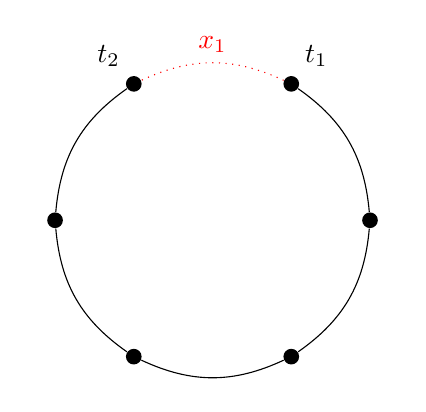
\begin{tikzpicture}[baseline]
 	 % Set the radius of the imaginary circle
 	 \def\radius{2cm}
 	 % Define the array of labels
 	 \def\labels{{4, 1, 2, 6, 5, 3}}
  
	  % Calculate the position of each point on the circle
 	 \foreach \i in {1,...,6} {
 	   \pgfmathsetmacro\label{\labels[\i - 1]}
 	   \ifthenelse{\label < 3}
 		    {\draw ({360/6 * (\i - 1)}:\radius) node[circle, fill, inner sep=2pt, label={360/6 * (\i - 1):$t_{\label}$}] (t\label) {};}
			{\draw ({360/6 * (\i - 1)}:\radius) node[circle, fill, inner sep=2pt, label={360/6 * (\i - 1)}:] (t\label) {};}
 	 }
  
 	 % Draw curved edges between specific points
 	 \draw (t4) to[out=95,in=-35] (t1);
 	 \draw (t2) to[out=215,in=85] (t6);
 	 \draw (t5) to[out=-25,in=205] (t3);
  
	 \draw[dotted, red] (t1) to[out=155,in=25] node[midway, above] {$x_1$} (t2);
	 \draw (t6) to[out=-85,in=145] (t5);
 	 \draw (t3) to[out=35,in=-95] (t4);
	\end{tikzpicture}
	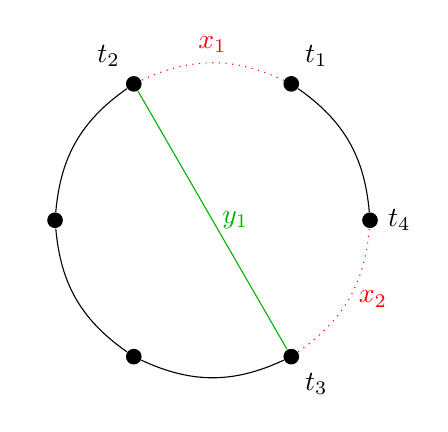
\begin{tikzpicture}[baseline]
 	 % Set the radius of the imaginary circle
 	 \def\radius{2cm}
 	 % Define the array of labels
 	 \def\labels{{4, 1, 2, 6, 5, 3}}
  
	  % Calculate the position of each point on the circle
 	 \foreach \i in {1,...,6} {
 	   \pgfmathsetmacro\label{\labels[\i - 1]}
 	   \ifthenelse{\label < 5}
 		    {\draw ({360/6 * (\i - 1)}:\radius) node[circle, fill, inner sep=2pt, label={360/6 * (\i - 1):$t_{\label}$}] (t\label) {};}
			{\draw ({360/6 * (\i - 1)}:\radius) node[circle, fill, inner sep=2pt, label={360/6 * (\i - 1)}:] (t\label) {};}
 	 }
  
 	 % Draw curved edges between specific points
 	 \draw (t4) to[out=95,in=-35] (t1);
 	 \draw (t2) to[out=215,in=85] (t6);
 	 \draw (t5) to[out=-25,in=205] (t3);
  
	 \draw[dotted, red] (t1) to[out=155,in=25] node[midway, above] {$x_1$} (t2);
	 \draw (t6) to[out=-85,in=145] (t5);
 	 \draw[dotted, red] (t3) to[out=35,in=-95] node[midway, right] {$x_2$} (t4);
 	 
	 \draw[green!70!black] (t2) to[] node[midway, right] {$y_1$} (t3);
	\end{tikzpicture}
	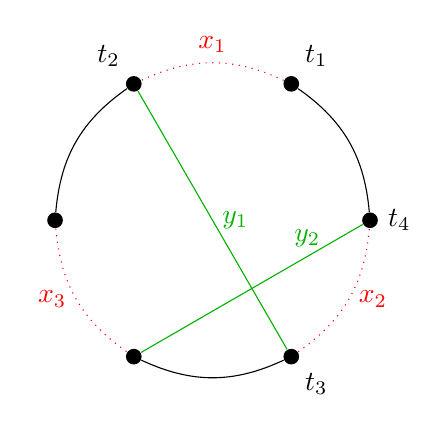
\begin{tikzpicture}[baseline]
 	 % Set the radius of the imaginary circle
 	 \def\radius{2cm}
 	 % Define the array of labels
 	 \def\labels{{4, 1, 2, 6, 5, 3}}
  
	  % Calculate the position of each point on the circle
 	 \foreach \i in {1,...,6} {
 	   \pgfmathsetmacro\label{\labels[\i - 1]}
 	   \ifthenelse{\label < 5}
 		    {\draw ({360/6 * (\i - 1)}:\radius) node[circle, fill, inner sep=2pt, label={360/6 * (\i - 1):$t_{\label}$}] (t\label) {};}
			{\draw ({360/6 * (\i - 1)}:\radius) node[circle, fill, inner sep=2pt, label={360/6 * (\i - 1)}:] (t\label) {};}
 	 }
  
 	 % Draw curved edges between specific points
 	 \draw (t4) to[out=95,in=-35] (t1);
 	 \draw (t2) to[out=215,in=85] (t6);
 	 \draw (t5) to[out=-25,in=205] (t3);
  
	 \draw[dotted, red] (t1) to[out=155,in=25] node[midway, above] {$x_1$} (t2);
	 \draw[dotted, red] (t6) to[out=-85,in=145] node[midway, left] {$x_3$} (t5);
 	 \draw[dotted, red] (t3) to[out=35,in=-95] node[midway, right] {$x_2$} (t4);
 	 
	 \draw[green!70!black] (t2) to[] node[midway, right] {$y_1$} (t3);
 	 \draw[green!70!black] (t4) to[] node[near start, above] {$y_2$} (t5);
	\end{tikzpicture}
	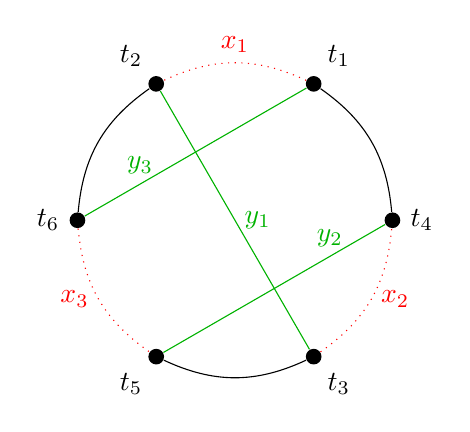
\begin{tikzpicture}[baseline]
 	 % Set the radius of the imaginary circle
 	 \def\radius{2cm}
 	 % Define the array of labels
 	 \def\labels{{4, 1, 2, 6, 5, 3}}
  
	  % Calculate the position of each point on the circle
 	 \foreach \i in {1,...,6} {
 	   \pgfmathsetmacro\label{\labels[\i - 1]}
 	   \draw ({360/6 * (\i - 1)}:\radius) node[circle, fill, inner sep=2pt, label={360/6 * (\i - 1):$t_{\label}$}] (t\label) {};
 	 }
  
 	 % Draw curved edges between specific points
 	 \draw (t4) to[out=95,in=-35] (t1);
 	 \draw (t2) to[out=215,in=85] (t6);
 	 \draw (t5) to[out=-25,in=205] (t3);
  
	  \draw[dotted, red] (t1) to[out=155,in=25] node[midway, above] {$x_1$} (t2);
	  \draw[dotted, red] (t6) to[out=-85,in=145] node[midway, left] {$x_3$} (t5);
 	 \draw[dotted, red] (t3) to[out=35,in=-95] node[midway, right] {$x_2$} (t4);
  
 	 \draw[green!70!black] (t1) to[] node[near end, above] {$y_3$} (t6);
	  \draw[green!70!black] (t2) to[] node[midway, right] {$y_1$} (t3);
 	 \draw[green!70!black] (t4) to[] node[near start, above] {$y_2$} (t5);
	\end{tikzpicture}
\end{center}
\captionof{figure}{Sekvenční hledání hran}\leavevmode\newline

Pro každou zrušenou hranu $x_i = (t_i, t_{i+1})$ hledáme hranu $y_i = (t_{i+1}, t_{i+2})$. Poslední přidaná hrana potom bude mít tvar $y_k = (t_{2i}, t_1)$.




Selection rule - rozdily delek, sequention
Stopping rule - Gi
Disjunction rule
Feasibility criterium


\subsubsection{Random info}
Rychlost cca $n ^ 2$

\begin{kiconclusions}
Závěr práce v \uv{českém} jazyce.
\end{kiconclusions}

\begin{kiconclusions}[english]
Thesis conclusions in \uv{English}.
\end{kiconclusions}


%% -------------------------------------------------------------------

%% Sazba volitelného seznamu zkratek, za přílohami.
\printglossary

%% Sazba povinné bibliografie, za přílohami (případně i za seznamem
%% zkratek). Při použití BibLaTeXu použijte makro
%% \printbibliography. jinak prostředí thebibliography. Ne obojí!

%% Sazba i v textu necitovaných zdrojů, při použití
%% BibLaTeXu. Volitelné.
\nocite{*}
%% Vlastní sazba bibliografie při použití BibLaTeXu.
\printbibliography

%% Bibliografie, včetně sazby, při nepoužití BibLaTeXu.
% \begin{thebibliography}{9}
%\bibitem{kniha2} \uppercase{Hawke}, Paul. NanoHttpd: Light-weight HTTP server designed for embedding in other applications. GitHub [online]. 2014-05-12. [cit. 2014-12-06]. Dostupné z: \url{https://github.com/NanoHttpd/nanohttpd}
%
%\bibitem{jeske13} \uppercase{Jeske}, David; \uppercase{Novák}, Josef. Simple HTTP Server in \csharp: Threaded synchronous HTTP Server abstract class, to respond to HTTP requests. CodeProject: For those who code [online]. 2014-05-24. [cit. 2014-12-06]. Dostupné z: \url{http://www.codeproject.com/Articles/137979/Simple-HTTP-Server-in-C}
%
%\bibitem{uzis2012} \uppercase{ÚSTAV ZDRAVOTNICKÝCH INFORMACÍ A STATISTIKY ČR}. Lékaři, zubní lékaři a farmaceuti 2012 [online]. Praha 2, Palackého náměstí 4: Ústav zdravotnických informací a statistiky ČR, 2012 [cit. 2014-12-06]. ISBN 978-80-7472-089-5. Dostupné z: \url{http://www.uzis.cz/publikace/lekari-zubni-lekari-farmaceuti-2012}
% \end{thebibliography}

%% Sazba volitelného rejstříku, za bibliografií.
\printindex

\end{document}

%%% Local Variables:
%%% mode: latex
%%% TeX-master: t
%%% End:
